%%%%%%%%%%%%%%%%%%%%%%%%%%%%%%%%%%%%%%%%%%%%%%%%%%%%%%%%%%%%%%%%%%%%%
%
% CSCI 1430 Written Question Template
%
% This is a LaTeX document. LaTeX is a markup language for producing documents. 
% You will fill out this document, compile it into a PDF document, then upload the PDF to Gradescope. 
%
% To compile into a PDF on department machines:
% > pdflatex thisfile.tex
%
% If you do not have LaTeX, your options are:
% - Use vscode! Install a distribution (all common OS): http://www.latex-project.org/get/ 
% + VSCode extension: https://marketplace.visualstudio.com/items?itemName=James-Yu.latex-workshop
% - Use an online tool: https://www.overleaf.com/ - most LaTeX packages are pre-installed here (e.g., \usepackage{}).
%
% If you need help with LaTeX, please come to office hours.
% Or, there is plenty of help online:
% https://en.wikibooks.org/wiki/LaTeX
%
% Good luck!
% The CSCI1430 staff
%
%%%%%%%%%%%%%%%%%%%%%%%%%%%%%%%%%%%%%%%%%%%%%%%%%%%%%%%%%%%%%%%%%%%%%

\documentclass{csci1430}

\begin{document}
\title{Homework 0 Questions}
\maketitle
\thispagestyle{fancy}

\writeinstructions

\section*{This Homework}
\begin{itemize}
  \item 7 questions \textbf{[4 + 4 + 8 + 6 + 5 + 3 + 3 = 33 points]}.
  \item Include code, images, and equations where appropriate.
\end{itemize}

\pagebreak % Please leave it here
%%%%%%%%%%%%%%%%%%%%%%%%%%%%%%%%%%%

\begin{question}[points=4]
For each of the following, complete the task and check the box to mark it as done.
\end{question}

%%% Complete the answerlist
\begin{answerlist}
    \item[\done] This is an example of a checked box.
    \item Read the GitHub tutorial \href{https://browncsci1430.github.io/resources/github_guide/}{here}.
    \item Create a GitHub account, if you don't have one.
    \item Join the \href{https://www.gradescope.com/}{Gradescope} course.
    \item Join the course \href{https://edstem.org/}{Ed}.
    \item Optionally \href{https://talktoata.com/join/brown-university-csci1430-spring-2025}{join ATA}.
    \item Complete the \href{https://colab.research.google.com/drive/1K42Mk-CPl8Azql5SJRE9xfkiNwRyo9rs?usp=sharing}{Python tutorial}.
    \item Set up the \href{https://browncsci1430.github.io/resources/python_setup/}{python environment and virtual environment}.
    \item Set up an editing environment (e.g.,~\href{https://browncsci1430.github.io/resources/vscode_setup/}{VSCode}), set it to use your python virtual environment, and know how to debug within it by setting breakpoints.
\end{answerlist}

\pagebreak % Please leave it here
%%%%%%%%%%%%%%%%%%%%%%%%%%%%%%%%%%%

\begin{question}[points=4]
Please find and read the course policies on the \href{https://browncsci1430.github.io/}{course website} and check whether each of the following scenarios violates the policy.
\end{question}

\begin{enumerate}[(a)]
\item
Search for Websites to help you clarify concepts, with citation in your submission.

% Remember: use \item[\done] to mark an answer.
\begin{answerlist}
    \item Acceptable
    \item Violation
\end{answerlist}

\item 
Ask ATA about a concept in the course, without citation in your submission.

\begin{answerlist}
    \item Acceptable
    \item Violation
\end{answerlist}   

\item 
Ask ChatGPT a question from the homework and submit its answer with minor changes, with citation in your submission.

\begin{answerlist}
    \item Acceptable
    \item Violation
\end{answerlist}

\item 
Look at another student's code before you write your own.

\begin{answerlist}
    \item Acceptable
    \item Violation
\end{answerlist}

\item
Talk to another CSCI 1430 student about your code to help you debug, after you have spent time trying to tackle the bug or have come to TA office hours/Ed.

\begin{answerlist}
    \item Acceptable
    \item Violation
\end{answerlist}

\item
Looking at code from a student who has previously taken the course to help you debug. The student is not a TA.

\begin{answerlist}
    \item Acceptable
    \item Violation
\end{answerlist}

\item
Using the result images from another student's code because your code has a bug.

\begin{answerlist}
    \item Acceptable
    \item Violation
\end{answerlist}

\end{enumerate}

\pagebreak % Please leave it here
%%%%%%%%%%%%%%%%%%%%%%%%%%%%%%%%%%%

\begin{question}[points=8,drawbox=false]
Computer vision is all around us, sometimes in surprising ways.
\end{question}

\begin{subquestion}[points=2]
If you could have any computer vision related superpower, with no limitations, what would it be and how would you use it? \textbf{[2-3 sentences]}
\end{subquestion}

\begin{answer}[height=7]

\end{answer}


\begin{subquestion}[points=6,drawbox=false]
All students enter the course with different backgrounds in socially responsible computing. Please first review our \href{https://browncsci1430.github.io/resources/ethics_primer/}{ethics primer} that introduces basic concepts to everyone.
\end{subquestion}

\begin{subsubquestion}[points=3]
State one value that is affected if you use your superpower. Explain your reasoning. \textbf{[2--3 sentences]}
\end{subsubquestion}
    
\begin{answer}[height=7]

\end{answer}


\begin{subsubquestion}[points=3]
State one value that is affected if your archenemy used your superpower. Explain your reasoning. \textbf{[2--3 sentences]}
\end{subsubquestion}
    
\begin{answer}[height=7]

\end{answer}

\pagebreak % Please leave it here
%%%%%%%%%%%%%%%%%%%%%%%%%%%%%%%%%%%

\begin{question}[points=6,drawbox=false]
Here is an image: \href{run:images/grizzlypeak-grayscale.png}{grizzlypeak-grayscale.png} (in the images directory)
\end{question}

\begin{subquestion}[drawbox=false]
Below is some code that sets pixels that have a value of 50 or less to 0. This removes some of the lower-intensity haze around the bright lights. However, the code only works on single-channel grayscale images.
\end{subquestion}

\begin{subsubquestion}[points=2]
Using another for loop and other appropriate modifications, convert the following code to work on \href{run:images/grizzlypeak-color.png}{grizzlypeak-color.png} (also in the images folder). You can paste the code in a Python file to run it. Make sure the conda env is activated.
\end{subsubquestion}

\begin{answer}[height=20]

TODO: Modify the following code:
\begin{python}
from skimage import io

A = io.imread('grizzlypeak-grayscale.png')
height, width = A.shape

# TODO: introduce a for loop that allows this 
# code to work on RGB images
for i in range(height):
    for j in range(width):
        if A[i,j] <= 50 :
            A[i,j] = 0
\end{python}
    
\end{answer}

\pagebreak
Let's find the time it takes to run this operation once. Because a single short task on multitasking computers often takes variable time, we can record how long code execution takes on a small number of images and then average the execution time.

\begin{subsubquestion}[points=1]
Record how long it takes on average by executing the program for 10 iterations and computing the mean time. Please include your code.
\end{subsubquestion}

\emph{Note: } When measuring the time, please ignore the file loading. You should only time the image modification itself.

\begin{answer}[height=30]
\begin{python}
# TODO: your code here
\end{python}

Report: How long does it take? TODO
\end{answer}

\pagebreak
\begin{subquestion}[points=3,drawbox=false]
Let's say we want to run our image modification 1000 times. If we used our current implementation, it would be slow. Let's suppose we can find a faster solution.
\end{subquestion}

\begin{subsubquestion}[points=2]
Using logical indexing (see the Python tutorial), find a faster solution to remove the haze. 
\end{subsubquestion}

\begin{answer}[height=25]
\begin{python}
# TODO: Your code here
\end{python}
\end{answer}


\pagebreak
\begin{subsubquestion}[points=1]
Now, using your optimized solution, record how long it takes to change the pixel values 1000 times. How long does the new code take to change the pixel values on one image? How much faster is the new version per image, as a
multiplicative factor (e.g., 2$\times$, 5$\times$)? Please include your code.
\end{subsubquestion}

\begin{answer}[height=30]
\begin{python}
# TODO: your code here
\end{python}

Report: How long does it take? TODO 

\end{answer}

\pagebreak % Please leave the pagebreak
%%%%%%%%%%%%%%%%%%%%%%%%%%%%%%%%%%%

\begin{question}[points=5,drawbox=false] 
Your friend tries to write code that reads an image into memory and displays it.
\end{question}
    
\begin{python}
from skimage import io
import matplotlib.pyplot as plt
import numpy as np

I = io.imread('./images/gigi.jpg').astype(np.float32)
plt.imshow(I)
plt.show()
\end{python}
    
However, when they run the code, the image is almost entirely white. Confused, they come to you for help.

\begin{subquestion}[points=1]
Why is the image being displayed incorrectly?\\
\emph{Hint: What data values does plt.imshow() expect?}
\end{subquestion}

\begin{answer}[height=6]

\end{answer}

\begin{subquestion}[points=2,drawbox=false]
You and your friend think of two possible ways to display the image correctly.
\end{subquestion}

\begin{subsubquestion}[points=1]
Write a possible fix that uses the float data type.
\end{subsubquestion}

\begin{answer}[height=10]
\begin{python}
# TODO: your code here
\end{python}
\end{answer}


\pagebreak % Please leave the pagebreak

\begin{subsubquestion}[points=1]
Write a possible fix that uses the 8-bit unsigned integer data type.
\end{subsubquestion}

\begin{answer}[height=10]
\begin{python}
# TODO: your code here
\end{python}
\end{answer}


\begin{subquestion}[points=2]
Your friend comes to you and wants help darkening an image.

Read in `gigi.jpg', darken all pixels by an amount equivalent to 20\% of the maximum brightness value of the \emph{pixel data type}, and display the new image. Include your code and a screenshot of the darkened image.
\end{subquestion}

\begin{answer}[height=23]
\begin{python}
# TODO: your code here - you can just write the critical lines
\end{python}

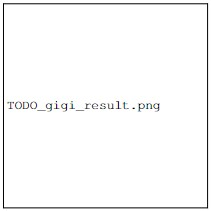
\includegraphics[width=0.5\textwidth,height=7cm,keepaspectratio]{images/TODO_gigi_result.jpg}
\end{answer}

\pagebreak
%%%%%%%%%%%%%%%%%%%%%%%%%%%%%%%%%%%

\begin{question}[points=3,drawbox=false]
The debugger within VSCode is an important tool you can use to discover potential bugs in the code that you write.

Imagine our task is to create a crop of an image that starts at the center of the image and extends to the lower right corner of the image. If all goes well, we should only see content from the lower right region of the original image.

\emph{Image:} \href{images/gigi.jpg}{gigi.jpg} (in images folder)

\begin{python}
from skimage import io
import matplotlib.pyplot as plt

origImage = io.imread('./images/gigi.jpg')
(height, width, channels) = origImage.shape
startCropX = width % 2
startCropY = height % 2
croppedImage = origImage[startCropY:, startCropX:]

plt.imshow(croppedImage)
plt.show()
\end{python}
\end{question}

\begin{orangebox}
Create a new python file in the same directory as the image, and copy in the above code block. Then, open the file in VSCode, and execute the code within a debugging session by pressing F5 (or `Run $\rightarrow$ Start Debugging'). At the prompt, we wish to `Debug the currently active Python file'.

The output is not currently what we want, so let's stop execution and then identify the bug in this program:
\begin{enumerate}[leftmargin=12pt,itemsep=2pt]
    \item First, set a breakpoint at line 7 and then re-execute the code for debugging.
    \item Inspect the `startCropX' variable either by looking at the left-hand Variables panel or by mouse hovering over the variable in the editor. What should it be?
    \item Execute line 7 of code by `stepping over' the current line (F10, or `Run $\rightarrow$ Step Over). We should now be about to execute line 8.
    \item Inspect `startCropY' and verify its correctness.
\end{enumerate}

At this point, you might have an idea of how to fix the code. But, before stopping execution and editing the file, let's test out our hypothesis in the `Debug Console' during debugging.
\end{orangebox}

\pagebreak
\begin{orangebox}
\begin{enumerate}[leftmargin=12pt,itemsep=2pt]
    \item Switch to the Debug Console by pressing CTRL-SHIFT-Y (or `View $\rightarrow$ Debug Console') --- you should see it in the bottom right of the display screen.
    \item \emph{This is an interactive Python console with access to working memory.} As a test, print out the value of `width'. Perform a mathematical operation on `width'.
    \item Assign the right value to `startCropX' within the Debug Console. Notice how the value updated in the Variables panel.
    \item Do the same for `startCropY'.
    \item From this point, execute the rest of the code by Continuing beyond our current paused position in the code. Press F5 to Continue (or `Run $\rightarrow$ Continue').
\end{enumerate}

Re-execute the debugger, and capture a screenshot showing your use of the Debug Console and inspection of a variable. Also, write the correct code below.
\end{orangebox}

\begin{answer}[height=30]
    %%%%%%% ANSWER STARTS HERE %%%%%%%%%%%%%%%%%%%%%%%%%%%%
    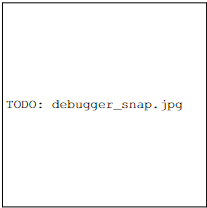
\includegraphics[width=0.5\textwidth,height=7cm,keepaspectratio]{images/TODO_debugger_snap.jpg}
    
    \begin{python}
    # TODO: paste your code here 
    \end{python}
    %%%%%%% ANSWER ENDS HERE %%%%%%%%%%%%%%%%%%%%%%%%%%%%
\end{answer}


\pagebreak
%%%%%%%%%%%%%%%%%%%%%%%%%%%%%%%%%%%

\begin{question}[points=3,drawbox=false]
This program should print out the maximum value in the matrix obtained by multiplying a random non-square matrix with its transpose.

Here, we're using some numpy functions that may be new to us, but they each have self-explanatory names.

\begin{python}
import numpy as np
from numpy import random as r

mat_1 = r.rand(200,150)
mat_2 = mat_1
np.transpose(mat_2)
mat_3 = np.matmul(mat_1, mat_2)
mat_max = np.max(mat_3)

print("Max value:", mat_max)
\end{python}
\end{question}

This time, when we execute the code, it will raise an exception.

\begin{orangebox}
Run the code in a debugging session, note the exception, and inspect the variables. Form a hypothesis for the error, set a breakpoint before it, and use the Debug Console to test that it prevents the exception. 
\end{orangebox}

\emph{Hint: Remember rules about matrix multiplication. What should the dimensions of each matrix be? Use the debugger to notice how the shapes of the images do or do not change.}

Capture a screenshot of your session showing us the issue and paste the correct code.

\begin{answer}[height=20]
    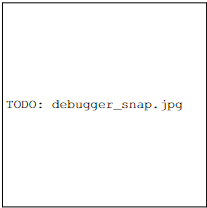
\includegraphics[width=0.5\textwidth,height=7cm,keepaspectratio]{images/TODO_debugger_snap.jpg}
    
    % Put the code on the next page.
\end{answer}

% Please leave the pagebreak
\pagebreak

\begin{answer}[height=30]
\begin{python}
# TODO: paste your code here
\end{python}
\end{answer}


\pagebreak
%%%%%%%%%%%%%%%%%%%%%%%%%%%%%%%%%%%

\section*{Feedback? (Optional)}
We appreciate your feedback on how to improve the course. You can provide anonymous feedback through \href{https://forms.gle/Eu5jJbDUmLknAyJV9}{this form} which can be accessed using your Brown account (your identity will not be collected). If you have urgent non-anonymous comments/questions, please email the instructor. 

\end{document}